% Author: Seongjin Lee 
% Gyeongsang National University, Korea 
% 
% 2021-02-14
%

\documentclass[newPxFont,sthlmFooter,nooffset]{beamer}
\usepackage{kotex, multicol}
%\usetheme{sthlm}
\usepackage{../style/beamerthemesthlm}
\hypersetup{pdfauthor={Seongjin Lee (insight@gnu.ac.kr)},
            pdfsubject={Data Structure and Algorithm, Lecture Note},
            pdfkeywords={Data Structure, Algorithm, Lecture, Note},
            pdfmoddate={D: \pdfdate},
            pdfcreator={Seongjin Lee}}

%\setbeamertemplate{footline}[text line]{%
%    \parbox{\linewidth}{\vspace*{-8pt} \insertsectionhead  \hfill\insertshortauthor\hfill\insertpagenumber}}
%\setbeamertemplate{navigation symbols}{}


\setbeamertemplate{blocks}[rounded]

\title{Data Structure and Algorithm}
\subtitle{Class 5}
\author[SJL]{Seongjin Lee}
\institute{\href{mailto:insight@gnu.ac.kr}{insight@gnu.ac.kr}\\\url{http://resourceful.github.io}\\Systems Research Lab.\\GNU}
\date{2021-02-14} 

\begin{document}



\frame[plain,t]{\titlepage} 

\frame{\frametitle{Table of contents}\tableofcontents} 


%---------------------------------------------------------
\section{Stack} 
\begin{frame}[t]
  \frametitle{Stack Abstract Data Type}
\textbf{Stack and Queue} is
\begin{itemize}
\item special cases of the more general data type, \textbf{Ordered List}
\end{itemize}

\textbf{ADT Stack}
\begin{itemize}
\item Ordered List
\item Insertions and deletions are made at one end called the top
\end{itemize}
\end{frame}

\begin{frame}[t]
  \frametitle{Stack Abstract Data Type}
Given stack $S = ( a_0, \ldots, a_{n-1})$
\begin{itemize}
\item $a_0$ : Bottom element
\item $a_{n-1}$ : Top element
\item $a_{i}$ : On top of element $a_{i-1}$ $(0 < i < n)$
\end{itemize}

A.K.A Last-In-First-out (LIFO)

\bigskip

Inserting and deleting elements in a stack
{\footnotesize  \begin{centering}
\begin{tabular}{!{\onslide<2->}c<{\onslide<3->}c<{\onslide<4->}c<{\onslide<5->}c<{\onslide<6->}c<{\onslide<7->}c}
push A & $\rightarrow$ push B &  $\rightarrow$ push C &  $\rightarrow$ push D &  $\rightarrow$ push E &  $\rightarrow$ pop E \\
    \end{tabular}
  \end{centering}}

{\onslide<1-> stack state}

{\footnotesize  \begin{centering}
\begin{tabular}{!{\onslide<2->} c<{\onslide<2->}c<{\onslide<3->}c<{\onslide<3->}c<{\onslide<4->}c<{\onslide<4->}c<{\onslide<5->}c<{\onslide<5->}c<{\onslide<6->}c<{\onslide<6->}c<{\onslide<7->}c<{\onslide<7->}c}
      & &   & &    &  &   &  & E & $\leftarrow$ top &   & \\
      & &   &  &   &  & D & $\leftarrow$ top & D  & & D &  $\leftarrow$ top\\
      & &   &  & C & $\leftarrow$ top & C  & & C & & C &\\
      & & B & $\leftarrow$ top & B & & B & & B & & B &\\
      A & $\leftarrow$ top & A & & A & & A & & A & & A &\\
    \end{tabular}
  \end{centering}}
\end{frame}

\begin{frame}[t]
  \frametitle{Stack Abstract Data Type: System Stack}
Stack is used by a program at run-time to process function calls

Activation record (stack frame) initially contains only 
\begin{itemize}
%typo revised -2021.02.11 kimsongsub-
\item a pointer to the previous stack frame
\item a return address
\end{itemize}
If this invokes another function
\begin{itemize}  
\item local variables
\item parameters of the invoking function
\end{itemize}

\end{frame}


\begin{frame}[t]
  \frametitle{Stack Abstract Data Type: System Stack}
System Stack after function call

{\onslide<2-> Run-time program simply creates a new stack frame
  \begin{itemize}
  \item also for each recursive call
  \end{itemize}
}

  \begin{center}
    \begin{tabular}{!{\onslide<1->}c<{\onslide<2->}c}
      \includegraphics[width=0.4\textwidth]{figures/fig03_stack1.png} &
      \includegraphics[width=0.4\textwidth]{figures/fig03_stack2.png} \\
    \end{tabular}
  \end{center}

\end{frame}
%add page -2021.02.13 kimsongsub-
\begin{frame}[t]
	\frametitle{Stack Abstract Data Type: System Stack}
	Frequent function calls may occupy all of the stack memory and may cause a stack overflow.
	\begin{center}
			
\includegraphics[width=0.4\textwidth]{figures/stackoverflow.png}
	\end{center}
%add source - 8p KSS-
\begin{tiny}
	\begin{flushright}
		The source of the picture is the ``Stack Overflow'' company's logo.
	\end{flushright}
\end{tiny}

\end{frame}


\begin{frame}[t,fragile]
  \frametitle{Stack Abstract Data Type}
\begin{codedef}
~\textbf{Structure:}~    Stack is 
   ~\textbf{Objects:}~ a finite ordered list with zero or more elements
   ~\textbf{Functions:}~
   For all stack ~$\in$~ Stack, 
   item ~$\in$~ element,
   max_stack_size ~$\in$~ positive integer:
       Stack CreateS(max_stack_size);
       Boolean IsFull(stack, max_stack_size);
       Stack Push(stack, item);
       Boolean IsEmpty(stack);
       Element Pop(stack); 
\end{codedef}
\end{frame}


\begin{frame}[t, fragile]
  \frametitle{Stack Abstract Data Type: Implementation}
  \begin{itemize}
  \item Using a one-dimensional array
    \begin{itemize}
    \item \texttt{stack[MAX\_STACK\_SIZE]}
    \item where \texttt{MAX\_STACK\_SIZE}: maximum number of entries
    \end{itemize}
  \end{itemize}
\begin{ncodedef}
#define MAX_STACK_SIZE  100
typedef struct {
    int key; // ~only key field~
             // ~can add/modify fields to meet the requirements~
} element;

element stack[MAX_STACK_SIZE];
int top = -1;
\end{ncodedef}
\end{frame}


\begin{frame}[t, fragile]
  \frametitle{Stack Abstract Data Type: implementation}
\texttt{IsEmpty(stack)}
  \begin{codedef}
    return(top < 0);
  \end{codedef}

\texttt{IsFull(stack);}

  \begin{codedef}
    return(top >= MAX_STACK_SIZE-1);
  \end{codedef}

\end{frame}


\begin{frame}[t, fragile]
  \frametitle{Stack Abstract Data Type: implementation}
\texttt{Push(stack, item)}

  \begin{codedef}
void push(int *ptop, element item){
    if (*ptop >= MAX_STACK_SIZE -1) {
       stack_full();
       return;
    }
    stack[++*ptop] = item;    
}
  \end{codedef}


\texttt{Pop(int *ptop);}

  \begin{codedef}
element pop(int *ptop){
    if(*ptop == -1)
        return stack_empty();
    return stack[(*ptop)--];
}
  \end{codedef}

\end{frame}

%add example -2021.02.13 kimsongsub-
\begin{frame}[t]
  \frametitle{Stack Abstract Data Type: Application of Stack}
  \begin{itemize}
  \item Procedure calls/returns
  \item Syntactic analyzer
  \item Converting non-recursive procedures to recursive procedures
  \item Save return address when calling subfunction
  \end{itemize}
\end{frame}




\section{Queues} 
\begin{frame}[t]
  \frametitle{Queue Abstract Data Type: Characteristics}
  \begin{itemize}
  \item Ordered list
  \item All insertions are made at one end, called \texttt{rear}
  \item All deletions are made at the other end, called \texttt{front}
  \item which item is to be removed first?
    \begin{itemize}
    \item \texttt{FIFO} (First In First Out)
    \end{itemize}
  \item All items except \texttt{front}/\texttt{rear} items are hidden
  \end{itemize}
\end{frame}

\begin{frame}[t]
  \frametitle{Queue Abstract Data Type:  Insertion and Deletion}

Operation
{\footnotesize  \begin{centering}
%typo revised delete D -> delete A -2021.02.12 kimsongsub-
\begin{tabular}{!{\onslide<2->}c<{\onslide<3->}c<{\onslide<4->}c<{\onslide<5->}c<{\onslide<6->}c}
insert A & $\rightarrow$ insert B &  $\rightarrow$ insert C &  $\rightarrow$ insert D &  $\rightarrow$ delete A  \\
    \end{tabular}
  \end{centering}}

{\onslide<1-> Queue state}

{\footnotesize  \begin{centering}
%front arrow location revised -2021.02.12 kimsongsub-
\begin{tabular}{!{\onslide<2->} c<{\onslide<2->}c<{\onslide<3->}c<{\onslide<3->}c<{\onslide<4->}c<{\onslide<4->}c<{\onslide<5->}c<{\onslide<5->}c<{\onslide<6->}c<{\onslide<6->}c}
       &                   &   &  &   &  & D & $\leftarrow$ rear & D & $\leftarrow$ rear \\
       &                   &   &  & C & $\leftarrow$ rear & C &  & C & \\
       &                   & B & $\leftarrow$ rear & B &  & B &  & B & $\leftarrow$ front\\
     A & $\leftarrow$ front, rear & A & $\leftarrow$ front & A & $\leftarrow$ front & A & $\leftarrow$ front &  & \\
    \end{tabular}
  \end{centering}}
\end{frame}

\begin{frame}[t, fragile]
  \frametitle{Queue Abstract Data Type: Implementation}
Simplest scheme
\begin{itemize}
\item one-dimensional array, and two variables: \texttt{front} and \texttt{rear}
\end{itemize}

\begin{ncodedef}
#define MAX_QUEUE_SIZE 100  
typedef struct {
    int key;
    /* other fields */
} element;

element queue[MAX_QUEUE_SIZE];
int rear = -1;
int front = -1;
\end{ncodedef}
\end{frame}

\begin{frame}[t, fragile]
  \frametitle{Queue Abstract Data Type: Implementation}
\texttt{IsEmptyQ(queue)}
\begin{codedef}
return (front == rear)
\end{codedef}
\texttt{IsFullQ(queue)}
\begin{codedef}
return rear == (MAX_QUEUE_SIZE-1)
\end{codedef}

\end{frame}

%add example -2021.02.13 kimsongsub-
\begin{frame}[t]
	\frametitle{Queue Abstract Data Type: Application of Queue}
	\begin{itemize}
		\item Buffer
		\item Job scheduling
	\end{itemize}
\end{frame}

\begin{frame}[t, fragile]
  \frametitle{Queue Abstract Data Type}
\texttt{addq(*prear, element item)}
\begin{ncodedef}
void addq(int *prear, element item){
    if(*prear == MAX_QUEUE_SIZE - 1){
        queue_full();
        return;
    }
    queue[++*prear] = item;
}
\end{ncodedef}

\texttt{deleteq(*pfront, int rear)}
\begin{ncodedef}
element deleteq(int *pfront, int rear){
    if(*pfront == rear){ // rear ~is used to check for an empty queue~
        return queue_empty();
    }
    return queue[++*pfront];
}
\end{ncodedef}
\end{frame}

\begin{frame}[t]
  \frametitle{Queue Abstract Data Type: Example - Sequential Queue}
\textbf{Job Scheduling}: Creation of job queue
\begin{itemize}
\item in the OS which does not use priorities, jobs are processed in the order they enter the system
\end{itemize}
\begin{tabular}{c | c | c c c c | l}
  front & rear & Q[0] & Q[1] & Q[2] & Q[3] & Comments \\ \hline \hline
    -1  &  -1  &      &      &      &      & Queue is empty \\
    -1  &   0  &  J1  &      &      &      & Job 1 is added \\
    -1  &   1  &  J1  &  J2  &      &      & Job 2 is added \\
    -1  &   2  &  J1  &  J2  &  J3  &      & Job 3 is added \\
     0  &   2  &      &  J2  &  J3  &      & Job 1 is deleted \\
     1  &   2  &      &      &  J3  &      & Job 2 is deleted \\
\end{tabular}
\end{frame}

\begin{frame}[t, fragile]
  \frametitle{Queue Abstract Data Type: Example - Sequential Queue}
\textbf{Problem}
\begin{itemize}
\item Queue gradually shifts to the right
\item \texttt{queue\_full(rear == MAX\_QUEUE\_SIZE-1)} signal does not
  always mean that there are MAX\_QUEUE\_SIZE items in queue
\item There may be empty spaces available
\item data movement: O(MAX\_QUEUE\_SIZE)
\end{itemize}
\bigskip
\textbf{Solution:}
  \begin{itemize}
  \item<2-> Circular Queue
  \end{itemize}
\end{frame}


\section{Circular Queues} 
\begin{frame}[t]
  \frametitle{Circular Queues}
More efficient Queue representation
\begin{itemize}
\item  regard the array \texttt{queue[MAX\_QUEUE\_SIZE]} as circular
\item initially \texttt{front} and \texttt{rear} to \texttt{0} rather than \texttt{-1}
\item the \texttt{front} index always points one position counterclockwise from the first element in the queue
\item the \texttt{rear} index point to the current end of the queue
\end{itemize}
\end{frame}

\begin{frame}[t]
  \frametitle{Circular Queues}
empty and nonempty circular queues
\includegraphics[width=0.9\textwidth]{figures/fig04_cq.png}
\end{frame}

\begin{frame}[t]
  \frametitle{Circular Queues}
full circular queues
\includegraphics[width=0.9\textwidth]{figures/fig05_fcq.png}
\end{frame}

%add quiz -2021.02.13 kimsongsub-
\begin{frame}[t]
	\frametitle{Circular Queues: Quiz}
What is the result ?
	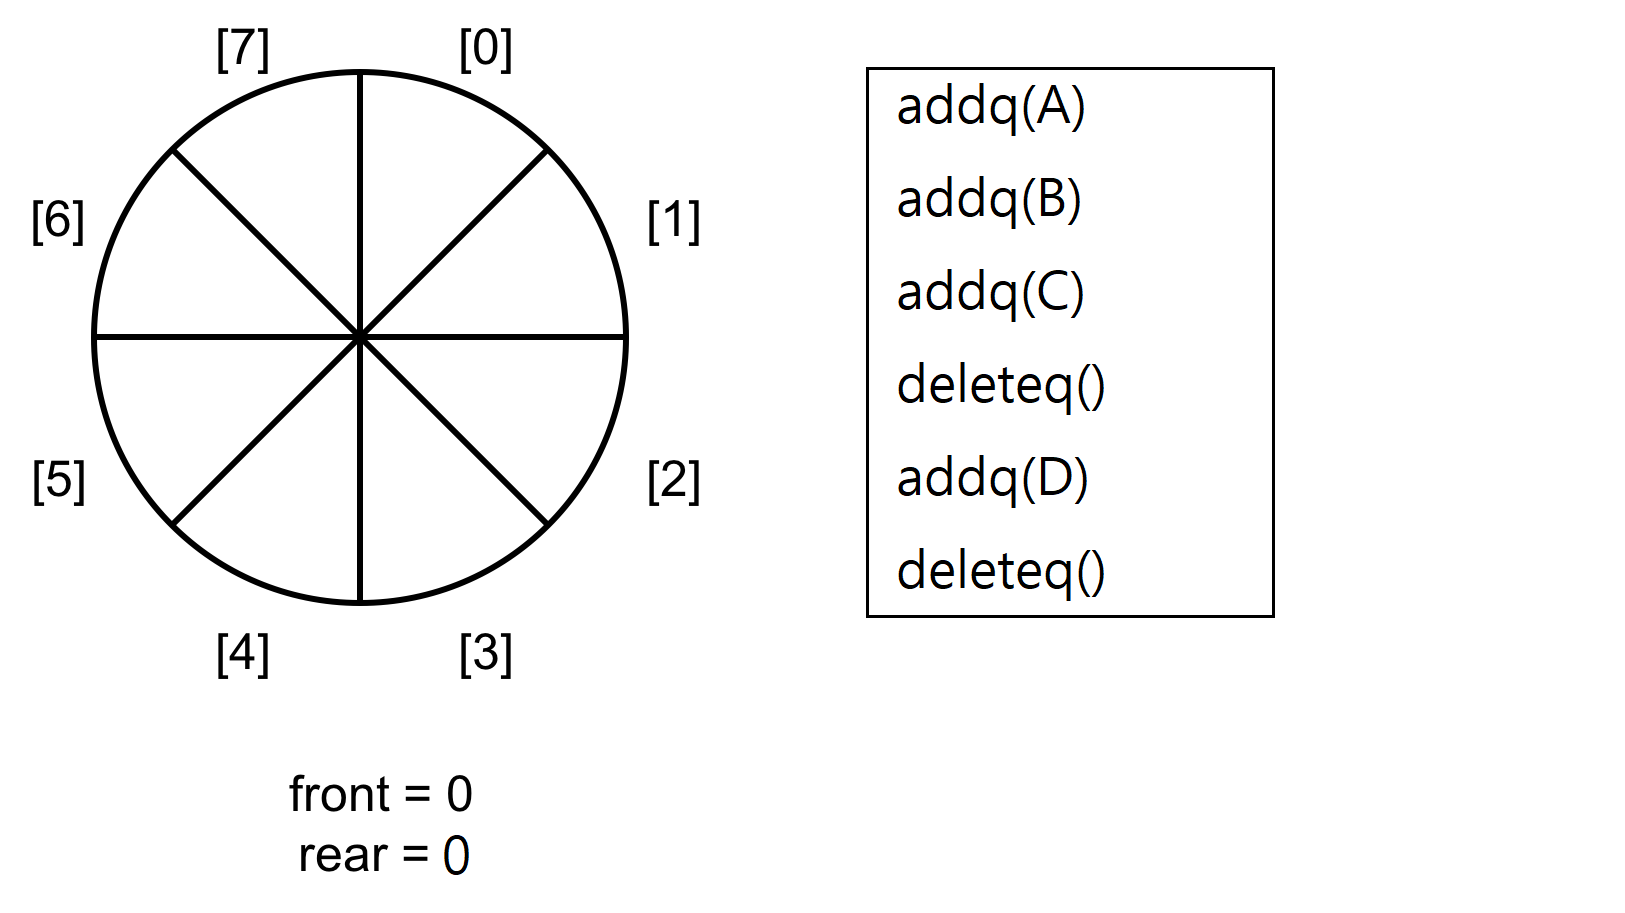
\includegraphics[width=0.9\textwidth]{figures/fig05_quiz1.png}
\end{frame}
%add quiz result -27p KSS-
\begin{frame}[t]
	\frametitle{Circular Queues: Quiz Result}
	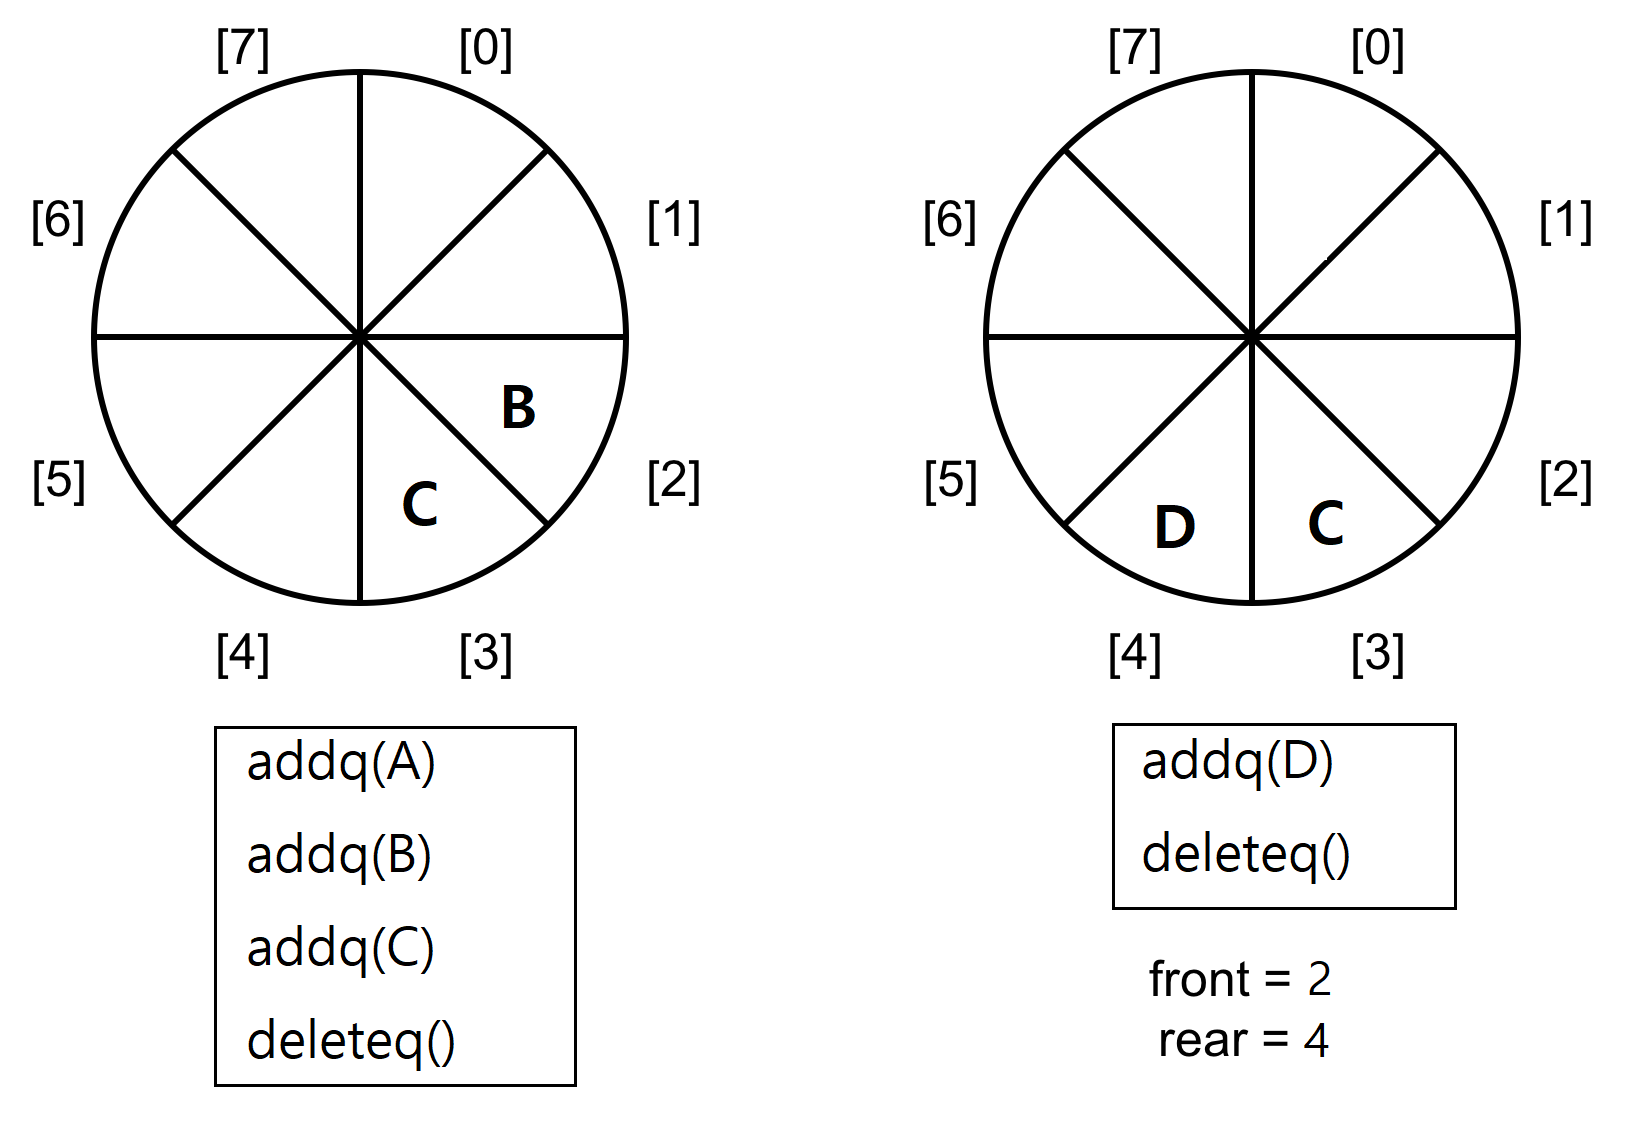
\includegraphics[width=0.9\textwidth]{figures/fig05_quiz2.png}
\end{frame}

%add quiz -2021.02.13 kimsongsub-
\begin{frame}[t, fragile]
	\frametitle{Circular Queues: Thinking}
	Why do not fill data in the empty space in front?

\begin{itemize}
	\item If all the data is filled in such a state, front and rear become the same, so it is impossible to distinguish whether it is empty or full.
	\item So, before all queue is filled, the size of the queue must be expanded.
\end{itemize}

\end{frame}

\begin{frame}[t, fragile]
  \frametitle{Circular Queues: Implementation}
  \begin{itemize}
  \item Use modulus operator for circular rotation
  \end{itemize}
\bigskip
\textbf{Circular rotation of the rear}
\begin{codedef}
rear = (rear + 1) % MAX_QUEUE_SIZE;
\end{codedef}

\textbf{Circular rotation of the front}
\begin{codedef}
front = (front + 1) % MAX_QUEUE_SIZE;
\end{codedef}
\end{frame}

\begin{frame}[t, fragile]
  \frametitle{Circular Queues: Implementation}
Add to a circular queue
\begin{itemize}
\item rotate rear before we place the item in the rear of the queue
\end{itemize}

\begin{ncodedef}
void addq(int front, int *prear, element item){
    *prear = (*prear + 1)  % MAX_QUEUE_SIZE;
    if (front == *prear) {
        queue_full(prear);
            /* reset rear and print error */
        return;
    }
    queue[*prear] = item;
}
\end{ncodedef}
\end{frame}

\begin{frame}[t, fragile]
  \frametitle{Circular Queues: Implementation}
Delete from a circular queue

\begin{ncodedef}
element deleteq(int *pfront, int rear){
    element item;
    if (*pfront == rear)
        return queue_empty();
        /* queue_empty returns an error key */
    *pfront = (*pfront + 1) % MAX_QUEUE_SIZE;
    return queue[*pfront];
}
\end{ncodedef}
\end{frame}

\begin{frame}[t]
  \frametitle{Circular Queues: Implementation notes}
Tests for a full queue and an empty queue are the same
\begin{itemize}
\item To distinguish between the case of full and empty, permit a maximum of \texttt{MAX\_QUEUE\_SIZE - 1}
\end{itemize}
\bigskip
No data movement necessary
\begin{itemize}
\item Ordinary queue: \texttt{O(n)}
\item Circular queue: \texttt{O(1)}
\end{itemize}

\end{frame}

\section{A Mazing Problem}
\begin{frame}[t]
  \frametitle{A Mazing Problem}
The representation of the maze
\begin{itemize}
\item two-dimensional array
\item element 0 : open path
\item element 1 : barriers
\end{itemize}
\includegraphics[width=0.7\textwidth]{figures/fig06_maze.png}
\end{frame}

\begin{frame}[t]
  \frametitle{A Mazing Problem: Allowable Movements}
\includegraphics[width=0.7\textwidth]{figures/fig07_moves.png}
\end{frame}

\begin{frame}[t]
  \frametitle{A Mazing Problem: Conditions}
\texttt{[row][col]} which is on border
\begin{itemize}
\item has only three (or two) neighbors
\item surround the maze by a border of 1's
\end{itemize}

\bigskip
\texttt{m*p} maze
\begin{itemize}
\item require $(m+2) *(p+2)$ array
\item entrance position: \texttt{[1][1]}
\item exit position: \texttt{[m][p]}
\end{itemize}
\end{frame}

\begin{frame}[t, fragile]
  \frametitle{A Mazing Problem: Data Type}
\begin{ncodedef}
typedef struct {
    short int vert;
    short int horiz;
} offsets

offsets move[8]; /* array of moves for each direction */    
\end{ncodedef}

\begin{tabular}{c | c | c | c}
  name & dir & \texttt{move[dir].vert} & \texttt{move[dir].horiz} \\ \hline
N  &  0 & -1 &  0 \\
NE &  1 & -1 &  1 \\
E  &  2 &  0 &  1 \\
SE &  3 &  1 &  1 \\
S  &  4 &  1 &  0 \\
SW &  5 &  1 &  -1 \\
W  &  6 &  0 &  -1 \\
NW &  7 & -1 &  -1 \\
\end{tabular}
\end{frame}

\begin{frame}[t, fragile]
  \frametitle{A Mazing Problem: Positioning of moves}
Position of next move
\begin{itemize}
\item move from current position: \texttt{maze[row][col]} to the next position \texttt{maze[next\_row][next\_col]}
\end{itemize}
\begin{ncodedef}
next_row = row + move[dir].vert;
next_col = col + move[dir].horiz;
\end{ncodedef}
\end{frame}

\begin{frame}[t]
  \frametitle{A Mazing Problem: Approach}
Maintain a second two-dimensional array, \texttt{mark}
\begin{itemize}
\item avoid returning to a previously tried path
\item initially, all entries are \texttt{0}
\item mark to 1 when the position is visited
\end{itemize}
\end{frame}

\begin{frame}[t, fragile]
  \frametitle{A Mazing Problem: Initial maze algorithm}
  \begin{ncodedef}
initialize a stack to the maze's entrance coordinates 
    and direction to north; 
while (stack is not empty) {
    /* move to position at top of stack */
    <row,col,dir> = delete from top of the stack;
    while (there are more moves from current position) { 
        <next_row, next_col> = coordinates of next move;
        dir = direction of move;
        if ((next_row == EXIT_ROW) && 
            (next_col == EXIT_COL)) 
            success;
        if (maze[next_row][next_col] == 0 && 
            mark[next_row][next_col] == 0) {
            mark[next_row][next_col] = 1;
            add <row, col, dir> to the top of the stack; 
            row = next_row;
            col = next_col;
            dir = north;
        } 
    }
}
printf("no path found\n");    
  \end{ncodedef}
\end{frame}

\begin{frame}[t, fragile]
  \frametitle{A Mazing Problem: Data Type}
\begin{ncodedef}
#define MAX_STACK_SIZE 100
typedef struct {
    short int row;
    short int col;
    short int dir;
} element;
element stack[MAX_STACK_SIZE];  
\end{ncodedef}

bound for the stack size
\begin{itemize}
\item the stack need only as many positions as there are zeroes in the maze
\end{itemize}
\end{frame}

\section{Evaluation of Expressions} 
\begin{frame}[t, fragile]
  \frametitle{Expressions}
  \begin{codedef}
    ~$x = a / b - c + d * e - a * c$~
  \end{codedef}
\bigskip

To understand the meaning of a expressions and statements
\begin{itemize}
\item figure out the order in which the operations are performed
\end{itemize}

Operator precedence hierarchy
\begin{itemize}
\item<determine the order to evaluate operators> 
\end{itemize}

associativity
\begin{itemize}
\item how to evaluate operators with the same precedence
\end{itemize}
\end{frame}


\begin{frame}[t]
  \frametitle{Precedence hierarchy for C}
{\footnotesize
  \begin{center}
  \begin{tabular}{c | c | c}
token & precedence & associativity \\ \hline
() [] -> . & 17 & left-to-right    \\
-\,- ++ & 16 & left-to-right    \\
-\,- ++ ! $\sim$ - + \& * sizeof & 15 & right-to-left \\
(type)  & 14 & right-to-left \\
* / \%  & 13 & left-to-right \\
+ -  & 12 & left-to-right \\
<< >> & 11 & left-to-right \\
> >= < <= & 10 & left-to-right \\
== !=  & 9 & left-to-right \\
\& & 8 & left-to-right \\
\string^ & 7 & left-to-right \\
$|$ & 6 & left-to-right \\
\&\&  & 5 & left-to-right \\
|| & 4 & left-to-right \\
?: & 3 & right-to-left \\
= += -= /= *= \%= <<= >>= \&= \string^= |= & 2 & right-to-left \\
, & 1 & left-to-right \\
  \end{tabular}
\end{center}
}
\end{frame}

\begin{frame}[t, fragile]
  \frametitle{Evaluation of Expressions}
\textbf{Human Style}
\begin{enumerate}
\item assign priority to each operator
\item use parenthesis and evaluate inner-most ones\\
     $(((A*(b+c))+(d/e))-(a/(c*d)))$
\end{enumerate}
\bigskip
\textbf{Compiler Style} (in postfix form)
\begin{enumerate}
\item translation (infix to postfix)
\item evaluation (postfix)
\end{enumerate}
\begin{codedef}
  prefix form: (operator) operand operand
  infix form: operand (operator) operand
  postfix form: operand operand (operator)
\end{codedef}
\end{frame}

\begin{frame}[t]
  \frametitle{Prefix, Infix, and Postfix Notation}
{\footnotesize  \begin{center}
    \begin{tabular}{c | c | c}
      Prefix & Infix & Postfix \\ \hline
 $+ 2~ * 3~ 4$  & $2+3*4$ & $2~ 3~ 4~* +$ \\
 $+ * a~ b~ 5$  & $a*b+5$ & $a~ b~ * 5~ +$\\
 $* + 1~ 2~ 7$  & $(1+2)*7$ & $1~ 2~ + 7~ *$ \\
 $/ * a~ b~ c$  & $a*b/c$ & $a~ b~ * c~ /$ \\
 $* / a~ + - b~ c~ d~ * - e~ a~ c$ 
    & $((a/(b-c+d))*(e-a)*c$ 
    & $a~ b~ c~ - d~ + / e~ a~ - * c~ *$ \\
$+ - / a~ b~ c~ - * d~ e~ * a~ c$ 
    & $a/b-c+d*e-a*c$ 
    & $a~b~/c~-d~e~*+a~c~*-$
    \end{tabular}
  \end{center}}
Evaluation of postfix expression
\begin{itemize}
\item scan left-to-right
\item place the operands on a stack until an operator is found
\item perform operations
\end{itemize}
\end{frame}

\begin{frame}[t]
  \frametitle{Evaluating Postfix Expression}
  \begin{center}
    $6~ 2~ / 3~ - 4~ 2~ * +$
  \end{center}

  \begin{center}
    \begin{tabular}{c | c c c | c}
      token & [0] & [1] & [2] & top \\ \hline
      6 & 6 &   &   & 0 \\
\onslide<2->      2 & 6 & 2 &   & 1 \\
\onslide<3->      / & 6/2 & & & 0 \\
\onslide<4->      3 & 6/2 & 3 & & 1 \\
\onslide<5->      - & 6/2-3 & & & 0 \\
\onslide<6->      4 & 6/2-3 & 4 & & 1 \\
\onslide<7->      2 & 6/2-3 & 4 & 2 & 2 \\
\onslide<8->      * & 6/2-3 & 4*2 & & 1 \\
\onslide<9->      + & 6/2-3+4*2 & & & 0 \\
    \end{tabular}
  \end{center}

\end{frame}

\begin{frame}[t]
  \frametitle{Evaluating Postfix Expression}
\texttt{get\_token()}
\begin{itemize}
\item used to obtain tokens from the expression string
\end{itemize}

\texttt{eval()}
\begin{itemize}
\item if the token is operand, convert it to number and push to the stack
\item otherwise
  \begin{itemize}
  \item pop two operands from the stack
  \item perform the specified operation
  \item push the result back on the stack
  \end{itemize}
\end{itemize}
\end{frame}


\begin{frame}[t, fragile]
  \frametitle{Evaluating of Expression}
\begin{ncodedef}
#define MAX_STACK_SIZE 100 /* maximum stack size */
#define MAX_EXPR_SIZE 100  /* max size of expression */

typedef enum {lparen, rparen, 
              plus, minus, 
              times, divide, 
              mode, eos, operand
             } precedence;  

int stack[MAX_STACK_SIZE]; /* global stack */
char expr[MAX_EXPR_SIZE];  /* input string */
\end{ncodedef}

represent stack by a global array
\begin{itemize}
\item accessed only through top
\item assume only the binary operator $+, -, *, /,$ and $\%$
\item assume single digit integer
\end{itemize}
\end{frame}

\begin{frame}[t, fragile, allowframebreaks]
   \frametitle{Function to evaluate a postfix expression}
\begin{ncodedef}
int eval(){
    precedence token;
    char symbol;

    int op1, op2;

    int n = 0;
    int top = -1;
  
    token = get_token(&symbol, &n); 
  
    while (token != eos) {
        if (token == operand)
            push(&top, symbol-’0’); 
        else {
            op2 = pop(&top); 
            op1 = pop(&top); 
  
            switch (token) {
                case plus: push(&top, op1+op2); 
                           break; 
                case minus: push(&top, op1-op2);
                           break; 
                case times: push(&top, op1*op2);
                           break; 
                case divide: push(&top, op1/op2);
                           break; 
                case mod: push(&top, op1%op2);
            } 
         }
         token = get_token(&symbol, &n); 
     }
     return pop(&top); 
}  
\end{ncodedef}

\end{frame}

\begin{frame}[t, fragile, allowframebreaks]
  \frametitle{Function to get a token}
  \begin{ncodedef}
precedence get_token(char *psymbol, int *pn) {
    *psymbol = expr[(*pn)++]; 
    switch (*psymbol)
        case ‘(‘ : return lparen;
        case ‘)‘ : return rparen;
        case ‘+‘ : return plus;
        case ‘-‘ : return minus;
        case ‘*‘ : return times;
        case ‘/‘ : return divide;
        case ‘%‘ : return mod;
        case ‘ ‘ : return eos;
        default : return operand; /* no error checking */
    } 
}    
  \end{ncodedef}
\end{frame}

\begin{frame}[t]
  \frametitle{Complexity}
  \begin{itemize}
  \item time: O(n) where n: number of symbols in expression
  \item space: stack \texttt{expr[MAX\_EXPR\_SIZE]}
  \end{itemize}
\end{frame}


\begin{frame}[t]
  \frametitle{Infix to Postfix}
Algorithm for producing a postfix expression from an infix one
\begin{enumerate}
\item fully parenthesize the expression
\item move all binary operators so that they replace their corresponding right parentheses
\item delete all parentheses
\end{enumerate}

e.g. $a/b-c+d*e-a*c$
\begin{enumerate}
\item $((((a/b)-c)+(d*e))-(a*c))$
\item ab/c-de*+ac*-
\end{enumerate}
\textit{Requires two pass}
\end{frame}

\begin{frame}[t]
  \frametitle{Infix to Postfix}
Form a postfix in one pass
\begin{itemize}
\item order of operands is the same in infix and postfix
\item order of operators depends on precedence
\item we can use stack
\end{itemize}

Simple expression: $a+b*c$
\begin{itemize}
\item $a~ b~ c~ * +$
\end{itemize}
\end{frame}

\begin{frame}[t]
  \frametitle{Infix to Postfix}
  \begin{itemize}
  \item Output operator with higher precedence before those with lower precedence
  \end{itemize}

\bigskip
Translation of $a+b*c$ to postfix
  \begin{center}
    \begin{tabular}{c | c c c | c | c}
      token & [0] & [1] & [2] & top & output \\ \hline
      a &  &   &   & -1 & a \\
\onslide<2->      + & + &  &  & 0 & a \\
\onslide<3->      b & + & & & 0 & ab \\
\onslide<4->      * & + & * & & 1 & ab \\
\onslide<5->      c & + & * & & 1 & abc \\
\onslide<6->      eos &  &  & & -1 & abc*+\\
    \end{tabular}
  \end{center}
\end{frame}

\begin{frame}[t]
  \frametitle{Infix to Postfix: Parenthesized expression}
parentheses make the translation process more difficult
\begin{itemize}
\item equivalent postfix expression is parenthesis-free
\end{itemize}

expression $a*(b+c)*d$
\begin{itemize}
\item yield $a~b~c+*d*$ in postfix
\end{itemize}

right parenthesis
\begin{itemize}
\item pop operators from a stack until left parenthesis is reached
\end{itemize}

\end{frame}

\begin{frame}[t]
  \frametitle{Infix to Postfix: Parenthesized expression}

Translation of $a*(b+c)*d$ to postfix
  \begin{center}
    \begin{tabular}{c | c c c | c | c}
      token & [0] & [1] & [2] & top & output \\ \hline
                  a &   &   &   & -1 & a \\
\onslide<2->      * & * &   &   & 0 & a \\
\onslide<3->      ( & * & ( &   & 1 & a \\
\onslide<4->      b & * & ( &   & 1 & ab \\
\onslide<5->      + & * & ( & + & 2 & ab \\
\onslide<6->      c & * & ( & + & 2 & abc \\
\onslide<7->      ) & * &   &   & 0 & abc+\\
\onslide<8->      * & * &   &   & 0 & abc+*\\
\onslide<9->      d & * &   &   & 0 & abc+*d\\
\onslide<10->   eos & * &   &   & 0 & abc+*d*\\
    \end{tabular}
  \end{center}
\end{frame}

\begin{frame}[t]
  \frametitle{Infix to Postfix}
A precedence-based scheme for stacking and unstacking operators
\begin{center}
  \includegraphics[width=0.7\textwidth]{figures/fig07_postfix.png}
\end{center}
\texttt{isp[stack[top]] < icp[token]} : push

\texttt{isp[stack[top]] $\geq$ icp[token]} : pop and print

\end{frame}

\begin{frame}[t, fragile]
  \frametitle{Infix to Postfix}
Use two types of precedence (because of the `(' operator)
\begin{itemize}
\item in-stack precedence (isp)
\item incoming precedence (icp)
\end{itemize}

\begin{ncodedef}
precedence stack[MAX_STACK_SIZE];
/* isp and icp arrays 
   -- index is value of precedence 
      lparen, rparen, plus, minus, 
      times divide, mode, eos */

static int isp[] = {0, 19, 12, 12, 13, 13, 13, 0};
static int icp[] = {20, 19, 12, 12, 13, 13, 13, 0};
\end{ncodedef}
\end{frame}

\begin{frame}[t, fragile, allowframebreaks]
  \frametitle{Infix to Postfix: the function}
Function to convert from infix to postfix
\begin{ncodedef}
void postfix(void) {
    char symbol;
    precedence token;
    int n = 0;
    int top = 0;
    stack[0] = eos;
    
    for (token = get_token(&symbol, &n); 
        token != eos; 
        token = get_token(&symbol, &n)) {

        if (token == operand) 
            printf("% c", symbol);
        else if (token == rparen) { 
            while (stack[top] != lparen) 
                print_token(pop(&top));

            pop(&top);
        } else {
            while (isp[stack[top]] >= icp[token]) 
                print_token(pop(&top));

            push(&top, token); 
        }
    }
    while ((token = pop(&top)) != eos)
        print_token(token); 

    printf("\n");
}
\end{ncodedef}
\end{frame}


\begin{frame}[t]
  \frametitle{Infix to Postfix}
postfix
\begin{itemize}
\item no parenthesis is needed
\item no precedence is needed
\end{itemize}

complexity
\begin{itemize}
\item time: O(r) where r: number of symbols in expression
\item space: S(n) = n where n: number of operators
\end{itemize}
\end{frame}

\begin{comment}
\section{Multiple Stacks Queues} 
\begin{frame}[t]
  \frametitle{Multiple Stacks and Queues}
\textbf{Multiple Stacks}

We need \textit{n} stacks simultaneously
\begin{itemize}
\item maximum size of each stack is unpredictable
\item size of each stack is dynamically varying
\item efficient memory utilization for multiple stacks is difficult
\end{itemize}
\end{frame}


\begin{frame}[t]
  \frametitle{Multiple Stacks and Queues}
Sequential mappings of stacks into an array
\begin{itemize}
\item \texttt{memory[MEM\_SIZE]}
\bigskip
\textbf{case n = 2}

The first stack:
\begin{itemize}
\item bottom element: \texttt{memory[0]}
\item grow toward \texttt{memory[MEM\_SIZE-1]}
\end{itemize}

The second stack:
\begin{itemize}
\item bottom element: \texttt{memory[MEM\_SIZE-1}
\item grow toward \texttt{memory[0]}
\end{itemize}
\end{itemize}

\end{frame}

\begin{frame}[t]
  \frametitle{Multiple Stacks and Queues}
  \begin{center}
    \includegraphics[width=0.8\textwidth]{figures/fig08_mulstack.png}
  \end{center}

\texttt{top[0] = -1}: stack 1 is empty

\texttt{top[1] = m}: stack 2 is empty
\end{frame}

\begin{frame}[t, fragile]
  \frametitle{Multiple Stacks and Queues: case n $\geq$ 3}
\begin{itemize}
\item \textit{boundary}: point to the position immediately to the left of the bottom element
\item \textit{top}: point to the top element
\end{itemize}
\begin{ncodedef}
#define MEM_SIZE 100
#define MAX_STACKS 10

element memory[MEM_SIZE];

int top[MAX_STACKS];
int boundary[MAX_STACKS];
int n; /* number of stacks, n < MAX_STACKS */
\end{ncodedef}
\end{frame}

\begin{frame}[t, fragile]
  \frametitle{Multiple Stacks and Queues: case n $\geq$ 3}
divide the array into roughly equal segments
\begin{ncodedef}
top[0] = boundary[0] = -1;
for(i = 1; i < n; i++)
    top[i] = boundary[i] = (MEM_SIZE/n)*i -1;
boundary[n] = MEM_SIZE -1;
\end{ncodedef}

  \begin{center}
    \includegraphics[width=0.8\textwidth]{figures/fig09_boundary.png}
  \end{center}
initial configuration for \textit{n} stacks in \texttt{memory[m]}
\end{frame}

\begin{frame}[t]
  \frametitle{Multiple Stacks and Queues: case n $\geq$ 3}
initially

\texttt{boundary[i] = top[i] = $\left\lfloor m/n\right\rfloor$ * i -1}

$i^{th}$ stack is empty
\begin{itemize}
\item \texttt{top[i] == boundary[i]}
\end{itemize}

$i^{th}$ stack is full
\begin{itemize}
\item \texttt{top[i] == boundary[i+1]}
\end{itemize}

\end{frame}

\begin{frame}[t, fragile]
  \frametitle{Multiple Stacks and Queues: case n $\geq$ 3}
push an item to the $i^{th}$ stack
\begin{ncodedef}
void push(int i, element item) { 
    /* add an item to the i-th stack */
    if (top[i] == boundary[i+1]) 
        stack_full(i);
    memory[++top[i]] = item; 
}    
\end{ncodedef}
\bigskip
pop an item from the $i^{th}$ stack
\begin{ncodedef}
element pop(int i) {
    /* remove top element from the i-th stack */
    if (top[i] == boundary[i]) 
        return stack_empty(i);
    return memory[top[i]--]; 
}
\end{ncodedef}
\end{frame}

\begin{frame}[t]
  \frametitle{Multiple Stacks and Queues: case n $\geq$ 3}
Ex. \texttt{n = 5, m = 20, push(1, x)}

\begin{center}
  \includegraphics[width=0.8\textwidth]{figures/fig10_ex.png}
\end{center}
\bigskip
\texttt{b[0]=-1 b[1]=3 b[2]=7 b[3]=11 b[4]=15}

\texttt{t[0]=-1 t[1]=7 t[2]=11 t[3]=13 t[4]=16}
\end{frame}

\begin{frame}[t]
  \frametitle{Multiple Stacks and Queues: case n $\geq$ 3}
  \begin{enumerate}
  \item find the least \texttt{j} for \texttt{i < j < n} such that there is a free space between stacks \texttt{j} and \texttt{(j+1)}
    \begin{itemize}
    \item i.e.) \texttt{t[j] < b[j+1]}
    \item move stack \texttt{i+1, i+2, ···,j} one position to the
      right creating a space between stacks \texttt{i} and
      \texttt{(i+1)}
    \end{itemize}
  \item if there is no such a j, then look up the left direction
  \item data movement: O(m)
  \end{enumerate}
\end{frame}
\end{comment}
\end{document}
